\documentclass{article}
\usepackage{graphicx} 
\usepackage{float}
\usepackage{booktabs}
\usepackage{array}
\usepackage{arydshln}
\usepackage{siunitx}
\usepackage{hyperref}
\usepackage{cancel}
\usepackage{changepage}
\usepackage{placeins}
\usepackage{enumitem}
\usepackage{siunitx}
%\usepackage{showframe}
\usepackage{times}

\usepackage{tabularx}
\usepackage{amsmath, amssymb, amscd, MnSymbol, mathrsfs}
\usepackage{cellspace}
\usepackage{tikz}
\usetikzlibrary{calc, patterns, angles, quotes, decorations.markings, decorations.pathmorphing, hobby}
\usepackage{xfrac}

\usepackage{chemfig}
\usepackage{caption}
\usepackage{tcolorbox}
\usepackage{bm}
\usepackage{pdfpages}
\usepackage{empheq}
\usepackage{pgfplots}
\pgfplotsset{compat=1.18}
\usepackage[oldvoltagedirection]{circuitikz}
\usepackage{microtype}
\usepackage{tikz-3dplot}
\usepackage{textcomp}
% Custom commands
\newcommand{\vect}[1]{\boldsymbol{\mathbf{#1}}}
\newcolumntype{C}{>{\centering\arraybackslash}X}
\newcolumntype{M}[1]{>{\centering\arraybackslash}m{#1}}

\usetikzlibrary{external}
\tikzexternalize[prefix=figures/]

\newcommand\myfrac[2]{\sfrac{#1\mkern-1.2mu}{#2}}
\usepackage{xcolor}

% Define custom colors
\definecolor{darkblue}{rgb}{0.1,0.1,0.5} % A dark blue shade
\definecolor{formalshade}{rgb}{0.95,0.95,1} % A light blue shade for the background

% For the adjustwidth environment
\PassOptionsToPackage{strict}{changepage}
\usepackage{changepage}

% For formal definitions
\usepackage{framed}

\newcommand{\formalsource}{} % Initialize an empty macro to store the source text

\newenvironment{formal}[3][]{% Start of the environment
	\renewcommand{\formalsource}{#1}% Store the optional argument
	\def\FrameCommand{%
		\hspace{1pt}%
		{\color{#2}\vrule width 2pt}%
		{\color{#3}\vrule width 4pt}%
		\colorbox{#3}%
	}%
	\MakeFramed{\advance\hsize-\width\FrameRestore}%
	\noindent\hspace{-4.55pt}% Disable indenting the first paragraph
	\begin{adjustwidth}{}{7pt}%
		\vspace{2pt}%
	}%
	{%
		\vspace{4pt}%
		\ifx\formalsource\empty % Check if the source is empty
		\else
		\hfill{\footnotesize{\formalsource}}% Align source to the bottom-right
		\fi
	\end{adjustwidth}\endMakeFramed%
}


% Custom itemize list with images for positive and negative items
\newlist{gitemize}{itemize}{1} % Just one level for the list
\setlist[gitemize,1]{
	leftmargin=2.8em, % Adjust the margin for the list
	labelsep=1em % Control the space between the label and the list item
}

% Define checkmark and cross symbols for positive and negative items
\newcommand{\checkitem}{\raisebox{-0.25\height}{\includegraphics[width=0.4cm]{checkmark.png}}}
\newcommand{\crossitem}{\raisebox{-0.25\height}{\includegraphics[width=0.4cm]{cross.png}}}


\usepackage[left=0.8in,right=0.8in,top=0.5in,bottom=0.69in,includeheadfoot,letterpaper]{geometry}
\usepackage{fancyhdr}
\usepackage{graphicx}
\usepackage{tabularray}
\usepackage{varwidth} 


\newcommand{\wm}[2]{%
	\begin{minipage}{#1\textwidth}
		\centering
		#2
	\end{minipage}%
}

\pagestyle{fancy}
\fancyhf{}


\renewcommand{\headrulewidth}{0.4pt}
\renewcommand{\footrulewidth}{0.4pt}

\fancyhead[L]{\includegraphics[height=1.2cm]{images/Kingston_University_London_logo_200-tablet.png}}
\fancyhead[R]{EG4024 – ME – Fluid Mechanics and Thermodynamics}
\fancyfoot[C]{Department of Mechanical Engineering}
\fancyfoot[R]{\thepage}

\usepackage{scalerel}

\setlength{\headheight}{30pt}
\setlength{\footskip}{20pt}



\usepackage[export]{adjustbox}
\usepackage{tocloft}
\renewcommand{\cfttoctitlefont}{}
\renewcommand{\contentsname}{}
\renewcommand{\cftsecleader}{\cftdotfill{\cftdotsep}}

\setlength{\cftbeforesecskip}{0.5em}


\usepackage{xcolor}      % For color options
\usepackage{hyperref}    % For hyperlinks
\usepackage{xurl}        % For better URL handling
\hypersetup{
	colorlinks=true,
	linkcolor=blue!50!black,
	urlcolor=blue,       % Color for URLs
}



%Refer to the equation as \eqref{equation}.
\usepackage{caption}  % This package allows captioning outside of a float
\usepackage[export]{adjustbox}


\usetikzlibrary{patterns}

\usetikzlibrary{patterns.meta}

\usepackage[para]{footmisc} % Example of making footnotes run together in a paragraph
\definecolor{darkgreen}{rgb}{0.0, 0.5, 0.0}  % Darker green

\usepackage{datetime}

\usepackage{xcolor}

\begin{document}
	
	\vspace*{\fill}
	\begin{center}
		\textbf{\Huge Laboratory Report}\\[10pt]
		\LARGE \textbf{Pressure \& Refrigeration}
	\end{center}
	\vspace*{\fill}
	
	\Large    
	\begin{tabular}{@{}l l l@{}}
		\textbf{Submitted by:} & Sakariye Abiikar & K2371673 \\
		& Alireza Alishahi & K2333243 \\
		& Naim Alrifai & K2459662 \\
		& Munachi J Atuegbu & K2463699 \\
		& Ehsan Haque & K2453799 \\
		& Abdul Mueed & K2454880 \\   
		& Abdelrahman Shehata & K2426523 \\   
		& Varley, Freddie & K2311322
	\end{tabular}
	
	\vspace*{\fill}
	
	\begin{tabular}{@{}l l@{}}
		\textbf{Key Dates:} & Date of practical: Wednesday 19$^{\text{th}}$ March, 2025 \\
		& Deadline: Tuesday 3$^{\text{rd}}$ April, 2025 \\
		& Last Updated: \today\, \currenttime\\
	\end{tabular}
	\vspace*{\fill}
	
	\large
	\newpage\noindent	\vspace*{-1em}
	
	\begin{center}
		\LARGE \textbf{Contribution Table}\\[3em]
	\end{center}	
	
	
	\begin{tblr}{
			colspec={Q[4cm]Q[4cm]Q[4cm]Q[3cm]},
			hlines,vlines,
			cells={valign=m,halign=c},
			rows={ht=4\baselineskip},
			row{1}={ht=1.5\baselineskip,font=\bfseries},
		}
		Student & Course & Contribution & Picture \\ 
		Sakariye Abiikar & Mechanical Engineering & ~ & \includegraphics[width=2cm,valign=c]{images/image(7).jpeg} \\ 
		Alireza Alishahi & Mechanical Engineering  & ~ & 
\includegraphics[width=2cm,valign=c]{images//profile.jpg} \\ 
		Naim Alrifai & Mechanical Engineering & ~ & 
\includegraphics[width=2cm,valign=c]{images/profile.jpg} \\ 
		Munachi J Atuegbu & Mechanical Engineering & ~  & 
\includegraphics[width=2cm,valign=c]{images//profile.jpg} \\ 
		Ehsan Haque & Mechanical Engineering & ~ & 
\includegraphics[width=2cm,valign=c]{images//profile.jpg} \\
		Abdul Mueed & Mechanical Engineering  & ~ & 
\includegraphics[width=2cm,valign=c]{images/profile.jpg} \\ 
		Abdelrahman Shehata & Mechanical Engineering  & ~ & 
\includegraphics[width=2cm,valign=c]{images/profile.jpg}\\
		Varley, Freddie & Mechanical Engineering & &  
\includegraphics[width=2cm,valign=c]{images/profile.jpg} 
	\end{tblr}
		\vspace*{\fill}
	
	\normalsize
	\newpage\newgeometry{top=0.2in,bottom=0.6in,left=0.8in,right=0.8in}
	\noindent\vspace{0em}
	\begin{center}
		\LARGE \textbf{Table of Contents}\\[-7em]
	\end{center}
	{
		\hypersetup{linkcolor=black}
		\tableofcontents
	}    
	
	
	\large\newpage\restoregeometry\vspace*{-20pt}
	
	\noindent
	
\section{Abstract}
In this experiment, we calibrated and compared the performance of multiple pressure-measuring devices, including two Bourdon gauges, a Budenberg pressure gauge and a Hg glass manometer, in tandem with a reference pressure calibrator (DPI-603 Portable Pressure Calibrator), which served as the baseline for pressure measurements and as the source of the applied pressure. The devices were connected to the DPI-603 Portable Pressure Calibrator, enabling us to apply both positive and negative pressures in increments of approximately $\pm$5 kPa. Through this process, we were able to get an exhaustive dataset that demonstrated notable differences in the pressure-measuring devices' performance. \textcolor{red!50!white}{[Placeholder breif results findings]}. These results highlighted the importance of selecting appropriate devices based on precision requirements and operating conditions, as well as the potential impact of human error in reading analog instruments like the Bourdon gauges and Hg manometer. 

	
	\newpage\vspace*{-20pt}

	\section{Introduction}
	In engineering and scientific applications, pressure measurement is essential, playing a critical role in fields such as fluid dynamics, meteorology, and industrial control. Over time, pressure-measuring instruments have evolved, from early liquid column manometers to modern mechanical and digital gauges, each designed to provide accurate measurements under varying conditions.\\[1em]
	A key distinction in pressure measurement is between \textbf{absolute} and \textbf{gauge} pressure \footnote{\textbf{differential} pressure i decided to redact in the context of our lab though it would be among this list}.\\ 
	Absolute pressure is measured relative to a vacuum, while gauge pressure is measured relative to atmospheric pressure. This distinction influences the design and function of pressure-measuring devices.\\[1em]
	Historically, the invention of the Bourdon gauge by Eugène Bourdon in 1849 marked a significant advancement in pressure measurement. It provided a robust and reliable means of monitoring pressure in industrial settings, where durability and consistency were paramount. On the other hand, liquid column manometers, particularly those using mercury, have been essential in laboratory settings due to their precision in measuring small pressure differences.\\[1em]
	Despite the advantages of different pressure-measuring devices, each has limitations, such as calibration errors and environmental influences.\\[1em]
	Previous studies have highlighted various challenges and findings related to pressure measurement devices. For example, a study by Hodgkinson et al. (2020) found that the accuracy of home blood pressure monitors varied significantly, with validated monitors showing a higher pass rate in static pressure tests compared to unvalidated ones. This emphasizes the importance of validation and calibration in ensuring the accuracy of pressure-measuring devices.\\[1em]
	In this experiment, we aimed to evaluate the performance and accuracy of various pressure-measuring devices under controlled conditions, comparing their responses to varying pressure levels.

	
	\newpage\vspace*{-20pt}
	\section{Method \& Experimental Procedures}\label{Method_Experimental_Procedures}
	We are first given a table to record our findings as shown:\footnote{We started of in the lab by doing the refrigerator but this is redacted as its not a part of this lab report, following this we did the pressure lab experiment.}
	\begin{figure}[H] 
		\centering 
		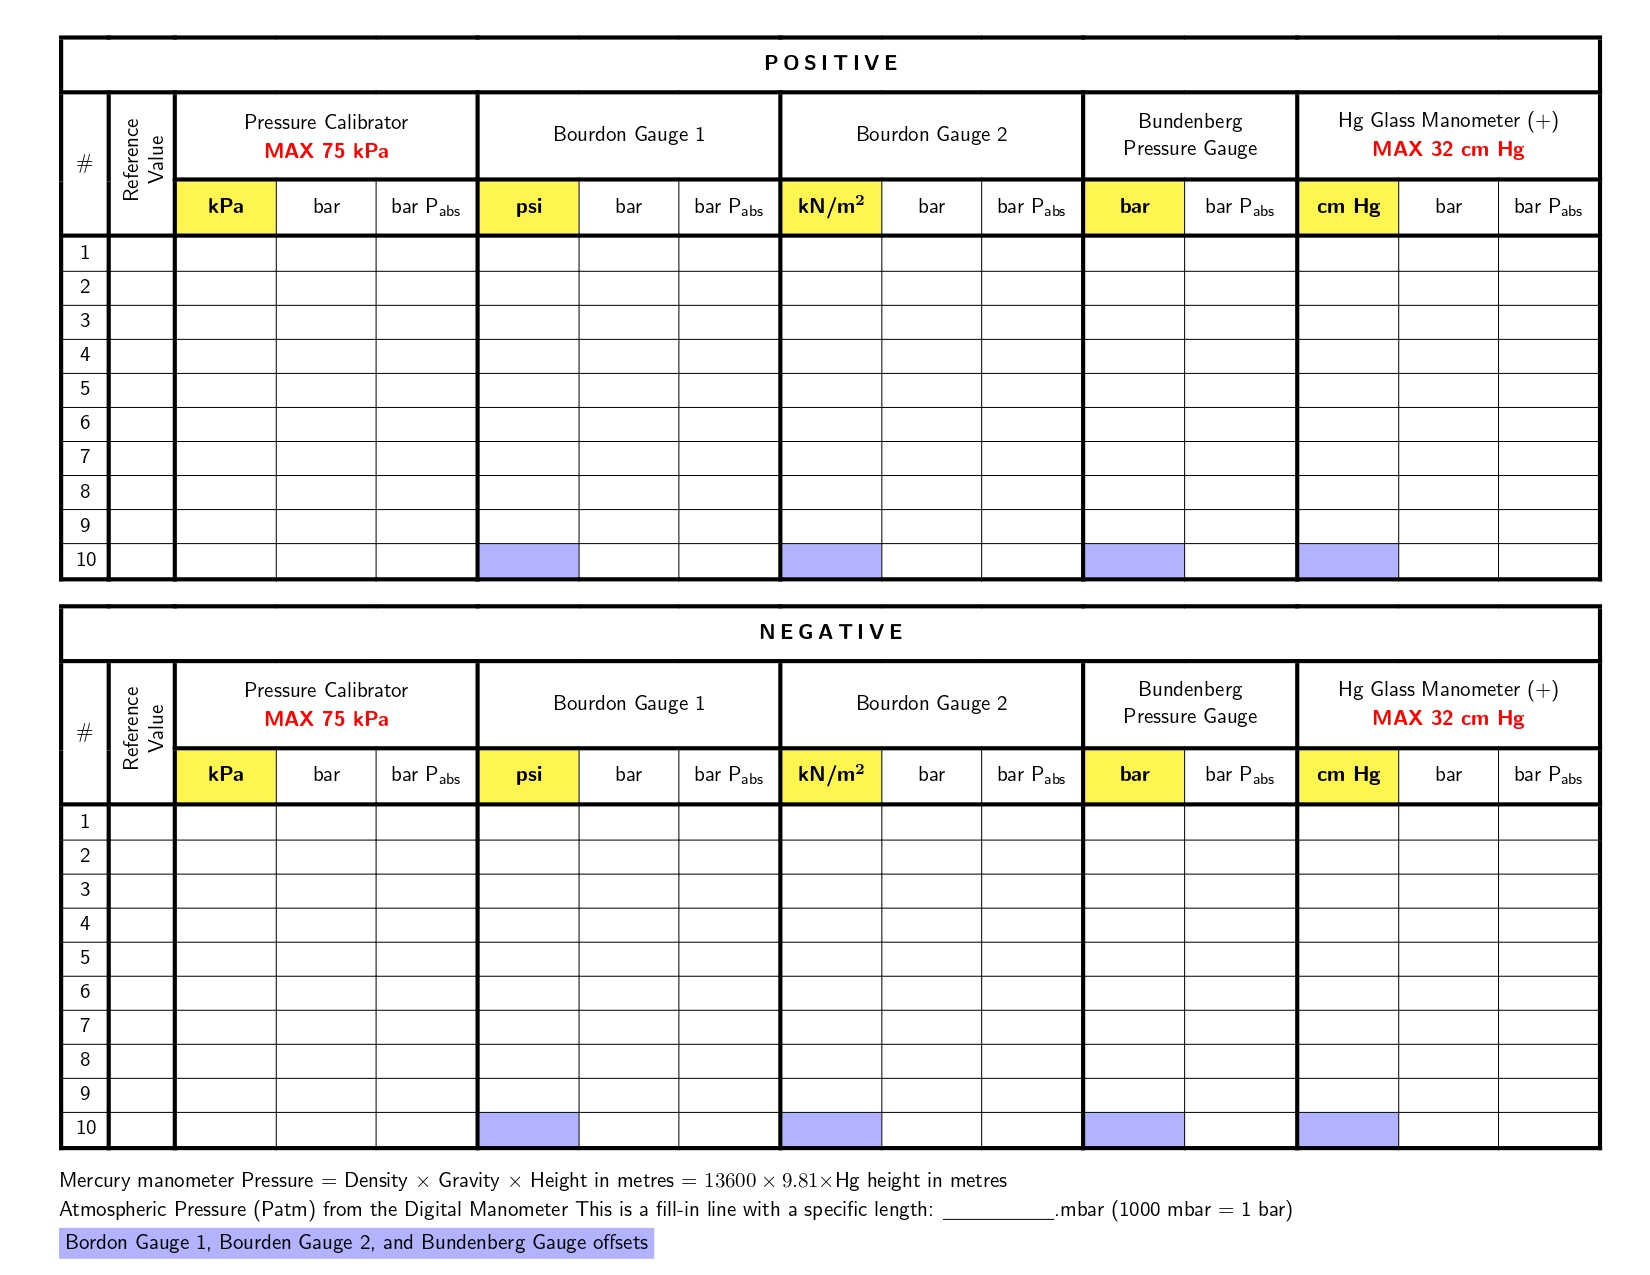
\includegraphics[width=1\textwidth,cfbox=gray!15 1pt]{images/tableland-1_page-0001.jpg} 
		\caption{Form for recording pressure measurements} 
		\label{fig:pressurestable} 
	\end{figure}
	We are then told the ropes of what the lab is, the steps we outlined as follows:
	\newpage
\hfil
\begin{minipage}{0.5\textwidth}	
	\subsection{Operating Procedure}
	\begin{enumerate}[left=0in,itemsep=2mm]
	\item Visual check test rigs pneumatic connections.
	\item Open the instruments vent valve.
	\item Select between positive (\textsf{\textcolor{red}{+}}) or negative (\textsf{\textcolor{blue}{-}}) as required. (This is the selector on the front of the DPI-603 ($\pm$VE on Figure \ref{fig:DPI-603}), located between the hand pump and the volume adjuster.)\\[5pt] We started with the positive pressure (Excess).
	\item Switch on the unit, pressing the power.
	\item Select Calibration Units, i.e., in Hg or bar, etc,\\[5pt] We went with kPa.
	\item  Close Vent valve and zero instrument using Vent Valve.\\[5pt] It was determined that due to the sensitivity of the vent valves, the instructure must perform this.
	\end{enumerate}
\end{minipage}\hfill
\begin{minipage}{0.45\textwidth}	
	\begin{figure}[H] 
		\centering 
		\begin{tikzpicture}[scale=0.5,transform shape]
			\node[anchor=center] (image) at (0,0) {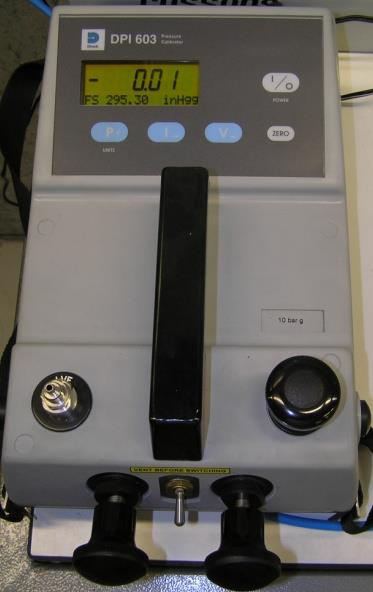
\includegraphics[width=1\textwidth]{extracted_images/image_8_1.png}};
			\draw[-{Latex[length=3mm,width=3mm]},line width=0.5mm] (3, -2) -- (5, -1) node[above=1mm,right] {\Huge Vent Valve}; 
			
			\draw[-{Latex[length=3mm,width=3mm]},line width=0.5mm] (-0.15, -5) -- (-0.15, -8) node[below=1mm] {\Huge $\pm \text{VE}$}; 
			
			\draw[-{Latex[length=3mm,width=3mm]},line width=0.5mm] (1.35, -6) -- (3, -8) node[below=6.5mm,right] {\Huge\text{Hand Pump}}; 
			
			\draw[-{Latex[length=3mm,width=3mm]},line width=0.5mm] (1.35-3, -6) -- (-3, -8) node[below=5.9mm,left] {\Huge\text{Volume Control}}; 
			
			\draw[-{Latex[length=3mm,width=3mm]},line width=0.5mm] (-2, 5) -- (-4, 7.5) node[above=5.9mm,left=-3cm] {\Huge\text{Calibration Units}}; 
			
			\draw[-{Latex[length=3mm,width=3mm]},line width=0.5mm,draw=black] (2.3, 4.8) -- (4.3, 7.4) node[above=5.9mm,right=-1cm] {\Huge\text{Power}}; 
		\end{tikzpicture}
		\caption{DPI-603 Portable Pressure Calibrator} 
		\label{fig:DPI-603} 
	\end{figure}
\end{minipage}\\
\begin{enumerate}
\item[7.] Using the hand pump pressurize the system to the required value ($\approx\pm 5$ kPa).\footnote{Caution is required when using the mercury (Hg) glass manometer. The maximum pressure should not exceed 32 cm Hg to prevent damage to the glass. In this experiment, pressure increments of 5 kPa were recorded, totaling 50 kPa, which remains safely within both the 32 cm Hg limit and the 75 kPa threshold. Therefore, the calibration was performed without exceeding the safe pressure limits.} Vent air using the vent valve and adjust pressure by pumping air using the hand pump. Use the volume control to fine-tune the pressure.
\item[7.] Once the required Obtain data from all relevant pressure gauges.

\item[9.] Reverse procedure for Vacuum.
\end{enumerate}

	
	\newpage
	\section{Theory}
	
	\newpage	
	\section{Data, Calculations and Results}
	Thus, as explained in the Method \& Experimental Procedures Section \ref{Method_Experimental_Procedures}, we have gathered a simple dataset for the corresponding pressure gauges. Our goal now is to make calculations, illustrate trends, etc., and simply produce another dataset from which we can draw fair conclusions from. Here, I first describe the baseline data that was collected and recorded on the table that was made available for use in the lab (Figure \ref{figure:s}).
	\subsection{Pressure Calibrator Readings}
	\vspace{-1em}
	\begin{table}[H]
		\centering
		\begin{minipage}[t]{0.17\textwidth}
			\centering
			\textbf{\textsf{kPa}}\\[8pt]
			
			\begin{tblr}{
					colspec={X[1cm]X[1cm]},
					hlines,vlines,
					cells={valign=m,halign=c},
					rows={ht=1\baselineskip},
					row{1}={ht=1\baselineskip,font=\bfseries},
				}
				\Large\textsf{\textcolor{red}{+}}&\wm{0.2}{\vspace{0.1cm}\Large\textsf{\textcolor{blue}{-}}}\\\hline
				0.0  & 0.0  \\
				5.7  & -5.6  \\
				10.4 & -12.1 \\
				16.0 & -18.0 \\
				21.1 & -21.8 \\
				27.7 & -25.4 \\
				34.2 & -29.3 \\
				40.0 & -33.6 \\
				46.1 & -37.6 \\
				52.2 & -41.7 \\
			\end{tblr}
			\caption{Pressure Calibrator}
		\end{minipage}
		\hfill
		\begin{minipage}[t]{0.17\textwidth}
			\centering
			\textbf{\textsf{psi}}\\[8pt]
			
			\begin{tblr}{
					colspec={X[1cm]X[1cm]},
					hlines,vlines,
					cells={valign=m,halign=c},
					rows={ht=1\baselineskip},
					row{1}={ht=1\baselineskip,font=\bfseries},
				}
				\Large\textsf{\textcolor{red}{+}}&\wm{0.2}{\vspace{0.1cm}\Large\textsf{\textcolor{blue}{-}}}\\\hline
				1.0  & 1.2  \\
				2.0  & 0.4  \\
				2.6  & -0.5  \\
				3.4  & -2.0  \\
				4.1  & -2.8  \\
				5.0  & -4.0  \\
				6.0  & -6.0  \\
				6.8  & -7.1  \\
				7.6  & -8.3  \\
				8.5  & -9.5  \\
			\end{tblr}
			\caption{Bourdon Gauge 1}
		\end{minipage}
		\hfill
		\begin{minipage}[t]{0.17\textwidth}
			\centering
			\textbf{\textsf{kN/m$\bm{^2}$}}\\[8pt]
			
			\begin{tblr}{
					colspec={X[1cm]X[1cm]},
					hlines,vlines,
					cells={valign=m,halign=c},
					rows={ht=1\baselineskip},
					row{1}={ht=1\baselineskip,font=\bfseries},
				}
				\Large\textsf{\textcolor{red}{+}}&\wm{0.2}{\vspace{0.1cm}\Large\textsf{\textcolor{blue}{-}}}\\\hline
				1.0  & 2.5  \\
				8.0  & -1.0  \\
				14.0 & -9.0  \\
				20.0 & -15.0 \\
				25.0 & -20.0 \\
				30.0 & -23.0 \\
				39.0 & -27.0 \\
				45.0 & -32.0 \\
				50.0 & -36.0 \\
				57.0 & -40.0 \\
			\end{tblr}
			\caption{Bourdon Gauge 2}
		\end{minipage}
		\hfill
		\begin{minipage}[t]{0.17\textwidth}
			\centering
			\textbf{\textsf{bar}}\\[8pt]
			
			\begin{tblr}{
					colspec={X[1cm]X[1cm]},
					hlines,vlines,
					cells={valign=m,halign=c},
					rows={ht=1\baselineskip},
					row{1}={ht=1\baselineskip,font=\bfseries},
				}
				\Large\textsf{\textcolor{red}{+}}&\wm{0.2}{\vspace{0.1cm}\Large\textsf{\textcolor{blue}{-}}}\\\hline
				-0.05 & -0.05  \\
				0.00  & -0.10  \\
				0.04  & -0.16  \\
				0.10  & -0.24  \\
				0.15  & -0.27  \\
				0.22  & -0.30  \\
				0.29  & -0.35  \\
				0.35  & -0.40  \\
				0.40  & -0.44  \\
				0.47  & -0.49  \\
			\end{tblr}
			\caption{Budenberg Pressure Gauge}
		\end{minipage}
		\hfill
		\begin{minipage}[t]{0.17\textwidth}
			\centering
			\textbf{\textsf{cm Hg}}\\[8pt]
			
			\begin{tblr}{
					colspec={X[1cm]X[1cm]},
					hlines,vlines,
					cells={valign=m,halign=c},
					rows={ht=1\baselineskip},
					row{1}={ht=1\baselineskip,font=\bfseries},
				}
				\Large\textsf{\textcolor{red}{+}}&\wm{0.2}{\vspace{0.1cm}\Large\textsf{\textcolor{blue}{-}}}\\\hline
				0.4  & 0.4  \\
				3.5  & -0.7  \\
				5.3  & -3.7  \\
				7.4  & -5.4  \\
				9.4  & -6.8  \\
				11.6 & -8.2  \\
				14.2 & -9.6  \\
				16.4 & -11.3 \\
				18.7 & -12.8 \\
				21.0 & -14.4 \\
			\end{tblr}
			\caption{Hg Glass Manometer}
		\end{minipage}
	\end{table}
	
	\newpage
	\section{Discussion of Results}
	
	\newpage\vspace*{-30pt}
	\section{Conclusions}
	\newpage\vspace*{-30pt}
	
	\section{Recommendations}  		
	\newpage\vspace*{-30pt}
	
	
	\section{References}		
	\newpage\vspace*{-30pt}
	
	\begin{enumerate}
		\item Hodgkinson, J.A. et al. (2020). \textit{Accuracy of blood-pressure monitors owned by patients with hypertension (ACCU-RATE study): a cross-sectional, observational study in central England}. British Journal of General Practice, [online] 70(697), pp.e548–e554. Available at: \url{https://bjgp.org/content/70/697/e548.}
	\end{enumerate}
	‌	
	
	\section{Appendix}
	
\end{document}
